\documentclass[../main.tex]{subfiles}
\begin{document}
		\chapter{Computing with finite elements}
	\label{chap:chap_13}
	%\pagenumbering{arabic}
	
	\noindent The purpose of this section is to demonstrate in detail how the finite element method can the be applied to the model problem
	$$
	-u^{\prime \prime}(x)=2, \quad x \in(0, L), u(0)=u(L)=0,
	$$
	with variational formulation
	$$
	\left(u^{\prime}, v^{\prime}\right)=(2, v) \quad \forall v \in V
	$$
	The variational formulation is derived in Section \ref{sec:sec_11_10}
	
	\section[Finite element mesh and basis functions]{Finite element mesh and basis functions}
		\label{sec:sec_13_1}
		
		\noindent We introduce a finite element mesh with $N_{e}$ cells, all with length $h$, and number the cells from left to right. global nodes. Choosing $\mathrm{P} 1$ elements, there are two nodes per cell, and the coordinates of the nodes become
		$$
		x_{i}=i h, \quad h=L / N_{e}, \quad i=0, \ldots, N_{n}=N_{e}+1,
		$$
		provided we number the nodes from left to right.\smallbreak
		Each of the nodes, $i$, is associated a finite element basis function $\varphi_{i}(x)$. When approximating a given function $f$ by a finite element function $u$, we expand $u$ using finite element basis functions associated with all nodes in the mesh, i.e., $N=N_{n}$. However, when solving differential equations we will often have $N<N_{n}$ because of Dirichlet boundary conditions. Why this is the case will now be explained in detail.\smallbreak
		In our case with homogeneous Dirichlet boundary conditions we do not need any boundary function $B(x)$ and can work with the expansion
		
		\begin{equation}
		\label{eqa170}
			u(x)=\sum_{j \in \mathcal{I}_{s}} c_{j} \psi_{j}(x) .
		\end{equation}
	
		\noindent Because of the boundary conditions, we must demand $\psi_{i}(0)=\psi_{i}(L)=0, i \in \mathcal{I}_{s}$. When $\psi_{i}, i=0, \ldots, N$, is to be selected among the finite element basis functions $\varphi_{j}, i=0, \ldots, N_{n}$, we have to avoid using $\varphi_{j}$ functions that do not vanish at $x_{0}=0$ and $x_{N_{n}}=L$. However, all $\varphi_{j}$ vanish at these two nodes for $j=1, \ldots, N_{n}$. Only basis functions associated with the end nodes, $\varphi_{0}$ and $\varphi_{N_{n}}$, violate the boundary conditions of our differential equation. Therefore, we select the basis functions $\varphi_{i}$ to be the set of finite element basis functions associated with all the interior nodes in the mesh:
		$$
		\psi_{i}=\varphi_{i+1}, \quad i=0, \ldots, N .
		$$
		Here, $N=N_{n}-2$.\smallbreak
		In the general case, the nodes are not necessarily numbered from left to right, so we introduce a mapping from the node numbering, or more precisely the degree of freedom numbering, to the numbering of the unknowns in the final equation system. These unknowns take on the numbers $0, \ldots, N$. Unknown number $j$ in the linear system corresponds to degree of freedom number $\nu(j)$, $j \in \mathcal{I}_{s}$. We can then write
		$$
		\psi_{i}=\varphi_{\nu(i)}, \quad i=0, \ldots, N .
		$$
		With a regular numbering as in the present example, $\nu(j)=j+1, j=1, \ldots, N=$ $N_{n}-2$.
	
	\section[Computation in the global physical domain]{Computation in the global physical domain}
		\label{sec:sec_13_2}
		\noindent We shall first perform a computation in the x coordinate system because the integrals can be easily computed here by simple, visual, geometric considerations.
		This is called a global approach since we work in the $x$ coordinate system and compute integrals on the global domain $[0, L]$.\smallbreak
		The entries in the coefficient matrix and right-hand side are
		$$
		A_{i, j}=\int_{0}^{L} \psi_{i}^{\prime}(x) \psi_{j}^{\prime}(x) \mathrm{d} x, \quad b_{i}=\int_{0}^{L} 2 \psi_{i}(x) \mathrm{d} x, \quad i, j \in \mathcal{I}_{s} .
		$$
		Expressed in terms of finite element basis functions $\varphi_{i}$ we get the alternative expressions
		$$
		A_{i, j}=\int_{0}^{L} \varphi_{i+1}^{\prime}(x) \varphi_{j+1}^{\prime}(x) \mathrm{d} x, \quad b_{i}=\int_{0}^{L} 2 \varphi_{i+1}(x) \mathrm{d} x, \quad i, j \in \mathcal{I}_{s} .
		$$
		For the following calculations the subscripts on the finite element basis functions are more conveniently written as $i$ and $j$ instead of $i+1$ and $j+1$, so our notation becomes
		$$
		A_{i-1, j-1}=\int_{0}^{L} \varphi_{i}^{\prime}(x) \varphi_{j}^{\prime}(x) \mathrm{d} x, \quad b_{i-1}=\int_{0}^{L} 2 \varphi_{i}(x) \mathrm{d} x
		$$
		where the $i$ and $j$ indices run as $i, j=1, \ldots, N_{n}-1=N+1$.\smallbreak
		The $\varphi_{i}(x)$ function is a hat function with peak at $x=x_{i}$ and a linear variation in $\left[x_{i-1}, x_{i}\right]$ and $\left[x_{i}, x_{i+1}\right]$. The derivative is $1 / h$ to the left of $x_{i}$ and $-1 / h$ to the right, or more formally,
	
		\begin{equation}
		\label{eqa171}
			\varphi_{i}^{\prime}(x)= \begin{cases}0, & x<x_{i-1}, \\ h^{-1}, & x_{i-1} \leq x<x_{i}, \\ -h^{-1}, & x_{i} \leq x<x_{i+1}, \\ 0, & x \geq x_{i+1}\end{cases}
		\end{equation}
	
		Figure \ref{fig:img_47} shows $\varphi_{1}^{\prime}(x)$ and $\varphi_{2}^{\prime}(x)$.
		\begin{figure}[H]
			\centering
			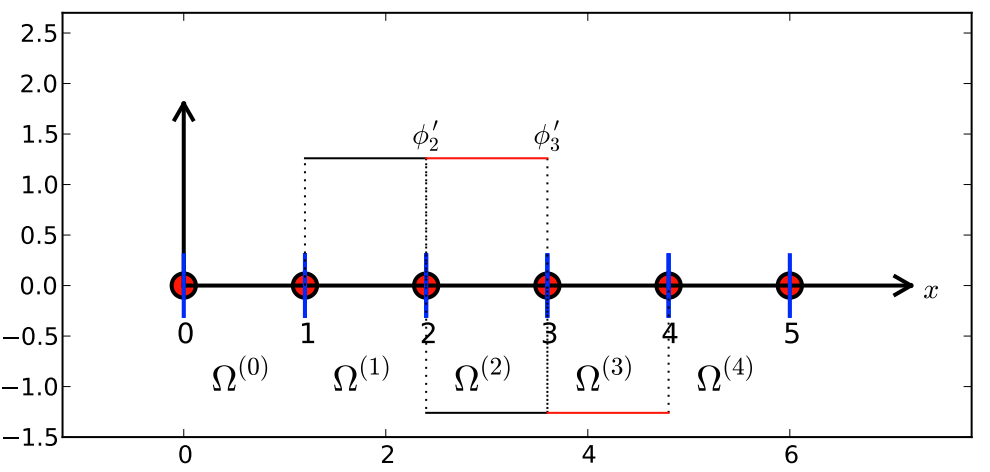
\includegraphics[width=0.7\linewidth]{img_47}
			\caption{Illustration of the derivative of piecewise linear basis functions associated with nodes in cell 2.}
			\label{fig:img_47}
		\end{figure}
		We realize that $\varphi_{i}^{\prime}$ and $\varphi_{j}^{\prime}$ has no overlap, and hence their product vanishes, unless $i$ and $j$ are nodes belonging to the same cell. The only nonzero contributions to the coefficient matrix are therefore
		$$
		\begin{aligned}
			A_{i-1, i-2} &=\int_{0}^{L} \varphi_{i}^{\prime}(x) \varphi_{i-1}^{\prime}(x) \mathrm{d} x, \\
			A_{i-1, i-1} &=\int_{0}^{L} \varphi_{i}^{\prime}(x)^{2} \mathrm{~d} x, \\
			A_{i-1, i} &=\int_{0}^{L} \varphi_{i}^{\prime}(x) \varphi_{i+1}^{\prime}(x) \mathrm{d} x,
		\end{aligned}
		$$
		for $i=1, \ldots, N_{n}-1$, but for $i=1, A_{i-1, i-2}$ is not defined, and for $i=N_{n}-1$, $A_{i-1, i}$ is not defined.
		
		We see that $\varphi_{i-1}^{\prime}(x)$ and $\varphi_{i}^{\prime}(x)$ have overlap of one cell $\Omega^{(i-1)}=\left[x_{i-1}, x_{i}\right]$ and that their product then is $-1 / h^{2}$. The integrand is constant and therefore $A_{i-1, i-2}=-h^{-2} h=-h^{-1}$. A similar reasoning can be applied to $A_{i-1, i}$, which also becomes $-h^{-1}$. The integral of $\varphi_{i}^{\prime}(x)^{2}$ gets contributions from two cells, $\Omega^{(i-1)}=\left[x_{i-1}, x_{i}\right]$ and $\Omega^{(i)}=\left[x_{i}, x_{i+1}\right]$, but $\varphi_{i}^{\prime}(x)^{2}=h^{-2}$ in both cells, and the length of the integration interval is $2 h$ so we get $A_{i-1, i-1}=2 h^{-1}$.
		
		The right-hand side involves an integral of $2 \varphi_{i}(x), i=1, \ldots, N_{n}-1$, which is just the area under a hat function of height 1 and width $2 h$, i.e., equal to $h$. Hence, $b_{i-1}=2 h$.
		
		To summarize the linear system, we switch from $i$ to $i+1$ such that we can write
		$$
		A_{i, i-1}=A_{i, i-1}=-h^{-1}, \quad A_{i, i}=2 h^{-1}, \quad b_{i}=2 h .
		$$
		
		The equation system to be solved only involves the unknowns $c_{i}$ for $i \in \mathcal{I}_{s}$. With our numbering of unknowns and nodes, we have that $c_{i}$ equals $u\left(x_{i+1}\right)$. The complete matrix system that takes the following form:
		
		\begin{equation}
		\label{eqa172}
			\frac{1}{h}\left(\begin{array}{ccccccccc}
				2 & -1 & 0 & \cdots & \cdots & \cdots & \cdots & \cdots & 0 \\
				-1 & 2 & -1 & \ddots & & & & & \vdots \\
				0 & -1 & 2 & -1 & \ddots & & & & \vdots \\
				\vdots & \ddots & & \ddots & \ddots & 0 & & & \vdots \\
				\vdots & & \ddots & \ddots & \ddots & \ddots & \ddots & & \vdots \\
				\vdots & & & 0 & -1 & 2 & -1 & \ddots & \vdots \\
				\vdots & & & & \ddots & \ddots & \ddots & \ddots & 0 \\
				\vdots & & & & & \ddots & \ddots & \ddots & -1 \\
				0 & \cdots & \cdots & \cdots & \cdots & \cdots & 0 & -1 & 2
			\end{array}\right)\left(\begin{array}{c}
				c_{0} \\
				\vdots \\
				\vdots \\
				\vdots \\
				\vdots \\
				\vdots \\
				\vdots \\
				\vdots \\
				c_{N}
			\end{array}\right)=\left(\begin{array}{c}
				2 h \\
				\vdots \\
				\vdots \\
				\vdots \\
				\vdots \\
				\vdots \\
				\vdots \\
				\vdots \\
				2 h
			\end{array}\right)
		\end{equation}
	
	\section[Comparison with a finite difference discretization]{Comparison with a finite difference discretization}
		\noindent A typical row in the matrix system can be written as
	
		\begin{equation}
		\label{eqa173}
			-\frac{1}{h} c_{i-1}+\frac{2}{h} c_{i}-\frac{1}{h} c_{i+1}=2 h .
		\end{equation}
	
		\noindent Let us introduce the notation $u_{j}$ for the value of $u$ at node $j: u_{j}=u\left(x_{j}\right)$ since we have the interpretation $u\left(x_{j}\right)=\sum_{j} c_{j} \varphi\left(x_{j}\right)=\sum_{j} c_{j} \delta_{i j}=c_{j}$. The unknowns $c_{0}, \ldots, c_{N}$ are $u_{1}, \ldots, u_{N_{n}}$. Shifting $i$ with $i+1$ in (173) and inserting $u_{i}=c_{i-1}$, we get
	
		\begin{equation}
		\label{eqa174}
			-\frac{1}{h} u_{i-1}+\frac{2}{h} u_{i}-\frac{1}{h} u_{i+1}=2 h,
		\end{equation}
	
		A finite difference discretization of $-u^{\prime \prime}(x)=2$ by a centered, second-order finite difference approximation $u^{\prime \prime}\left(x_{i}\right) \approx\left[D_{x} D_{x} u\right]_{i}$ with $\Delta x=h$ yields
	
		\begin{equation}
		\label{eqa175}
			-\frac{u_{i-1}-2 u_{i}+u_{i+1}}{h^{2}}=2,
		\end{equation}
		which is, in fact, equivalent to (174) if (174) is divided by $h$. Therefore, the finite difference and the finite element method are equivalent in this simple test problem.
		
		Sometimes a finite element method generates the finite difference equations on a uniform mesh, and sometimes the finite element method generates equations that are different. The differences are modest, but may influence the numerical quality of the solution significantly, especially in time-dependent problems.\bigbreak 
		
\section[Cellwise computations]{Cellwise computations}
	\label{sec:sec_13_4}
	\noindent We now employ the cell by cell computational procedure where an element matrix and vector are calculated for each cell and assembled in the global linear system. All integrals are mapped to the local reference coordinate system $X \in[-1,1]$. In the present case, the matrix entries contain derivatives with respect to $x$,
	$$
	A_{i-1, j-1}^{(e)}=\int_{\Omega^{(\varepsilon)}} \varphi_{i}^{\prime}(x) \varphi_{j}^{\prime}(x) \mathrm{d} x=\int_{-1}^{1} \frac{d}{d x} \tilde{\varphi}_{r}(X) \frac{d}{d x} \tilde{\varphi}_{s}(X) \frac{h}{2} \mathrm{~d} X,
	$$
	where the global degree of freedom $i$ is related to the local degree of freedom $r$ through $i=q(e, r)$. Similarly, $j=q(e, s)$. The local degrees of freedom run as $r, s=0,1$ for a P1 element.\bigbreak

	\textbf{The integral for the element matrix.  } There are simple formulas for the basis functions $\tilde{\varphi}_{r}(X)$ as functions of $X$. However, we now need to find the derivative of $\tilde{\varphi}_{r}(X)$ with respect to $x$. Given
	$$
	\tilde{\varphi}_{0}(X)=\frac{1}{2}(1-X), \quad \tilde{\varphi}_{1}(X)=\frac{1}{2}(1+X),
	$$
	we can easily compute $d \tilde{\varphi}_{r} / d X$ :
	$$
	\frac{d \tilde{\varphi}_{0}}{d X}=-\frac{1}{2}, \quad \frac{d \tilde{\varphi}_{1}}{d X}=\frac{1}{2}
	$$
	From the chain rule,
	
	\begin{equation}
		\label{eqa176}
		\frac{d \tilde{\varphi}_{r}}{d x}=\frac{d \tilde{\varphi}_{r}}{d X} \frac{d X}{d x}=\frac{2}{h} \frac{d \tilde{\varphi}_{r}}{d X}
	\end{equation}	

	\noindent The transformed integral is then
	$$
	A_{i-1, j-1}^{(e)}=\int_{\Omega(\varepsilon)} \varphi_{i}^{\prime}(x) \varphi_{j}^{\prime}(x) \mathrm{d} x=\int_{-1}^{1} \frac{2}{h} \frac{d \tilde{\varphi}_{r}}{d X} \frac{2}{h} \frac{d \tilde{\varphi}_{s}}{d X} \frac{h}{2} \mathrm{~d} X
	$$
	\textbf{The integral for the element vector.  } The right-hand side is transformed according to
	$$
	b_{i-1}^{(e)}=\int_{\Omega(e)} 2 \varphi_{i}(x) \mathrm{d} x=\int_{-1}^{1} 2 \tilde{\varphi}_{r}(X) \frac{h}{2} \mathrm{dX}, \quad i=q(e, r), r=0,1
	$$
	\textbf{Detailed calculations of the element matrix and vector.   } Specifically for P1 elements we arrive at the following calculations for the element matrix entries:
	$$
	\begin{aligned}
		\tilde{A}_{0,0}^{(e)} &=\int_{-1}^{1} \frac{2}{h}\left(-\frac{1}{2}\right) \frac{2}{h}\left(-\frac{1}{2}\right) \frac{2}{h} \mathrm{~d} X=\frac{1}{h} \\
		\tilde{A}_{0,1}^{(e)} &=\int_{-1}^{1} \frac{2}{h}\left(-\frac{1}{2}\right) \frac{2}{h}\left(\frac{1}{2}\right) \frac{2}{h} \mathrm{~d} X=-\frac{1}{h} \\
		\tilde{A}(e) &=\int_{1,0}^{1} \frac{2}{h}\left(\frac{1}{2}\right) \frac{2}{h}\left(-\frac{1}{2}\right) \frac{2}{h} \mathrm{~d} X=-\frac{1}{h} \\
		\tilde{A}_{1,1}^{(e)} &=\int_{-1}^{1} \frac{2}{h}\left(\frac{1}{2}\right) \frac{2}{h}\left(\frac{1}{2}\right) \frac{2}{h} \mathrm{~d} X=\frac{1}{h}
	\end{aligned}
	$$
	The element vector entries become
	$$
	\begin{aligned}
		&\tilde{b}_{0}^{(e)}=\int_{-1}^{1} 2 \frac{1}{2}(1-X) \frac{h}{2} \mathrm{~d} X=h \\
		&\tilde{b}_{1}^{(e)}=\int_{-1}^{1} 2 \frac{1}{2}(1+X) \frac{h}{2} \mathrm{~d} X=h
	\end{aligned}
	$$
	Expressing these entries in matrix and vector notation, we have
	\begin{equation}
			\label{eqa177}
		\tilde{A}^{(e)}=\frac{1}{h}\left(\begin{array}{rr}
			1 & -1 \\
			-1 & 1
		\end{array}\right), \quad \tilde{b}^{(e)}=h\left(\begin{array}{l}
			1 \\
			1
		\end{array}\right)
	\end{equation}

	\noindent \textbf{Contributions from the first and last cell.   } The first and last cell involve only one unknown and one basis function because of the Dirichlet boundary conditions at the first and last node. The element matrix therefore becomes a $1 \times 1$ matrix and there is only one entry in the element vector. On cell 0 , only $\psi_{0}=\varphi_{1}$ is involved, corresponding to integration with $\tilde{\varphi}_{1}$. On cell $N_{e}$, only $\psi_{N}=\varphi_{N_{n}-1}$ is involved, corresponding to integration with $\tilde{\varphi}_{0}$. We then get the special end-cell contributions
	
	\begin{equation}
		\label{eqa178}
		\tilde{A}^{(e)}=\frac{1}{h}(1), \quad \tilde{b}^{(e)}=h(1),
	\end{equation}

	for $e=0$ and $e=N_{e}$. In these cells, we have only one degree of freedom, not two as in the interior cells.\bigbreak
	
	\noindent \textbf{Assembly.   } The next step is to assemble the contributions from the various cells. The assembly of an element matrix and vector into the global matrix and right-hand side can be expressed as
	$$
	A_{q(e, r), q(e, s)}=A_{q(e, r), q(e, s)}+\tilde{A}_{r, s}^{(e)}, \quad b_{q(e, r)}=b_{q(e, r)}+\tilde{b}_{r}^{(e)},
	$$
	for $r$ and $s$ running over all local degrees of freedom in cell $e$.\smallbreak
	To make the assembly algorithm more precise, it is convenient to set up Python data structures and a code snippet for carrying out all details of the algorithm. For a mesh of four equal-sized P1 elements and $L=2$ we have
	\begin{lstlisting}[numbers=none]
		vertices =[0,0.5,1,1.5,2]
		cells =[[0,1],[1,2],[2,3],[3,4]]
		dof_map =[[0],[0,1],[1,2],[2]]
	\end{lstlisting}
	The total number of degrees of freedom is 3 , being the function values at the internal 3 nodes where $u$ is unknown. In cell 0 we have global degree of freedom 0 , the next cell has $u$ unknown at its two nodes, which become global degrees of freedom 0 and 1 , and so forth according to the \textbf{\texttt{dof\_map}} list. The mathematical $q(e, r)$ quantity is nothing but the \textbf{\texttt{dof\_map}} list.
	Assume all element matrices are stored in a list \textbf{\texttt{Ae}} such that \textbf{\texttt{Ae[e][i, j]}} is $\tilde{A}_{i, j}^{(e)}$. A corresponding list for the element vectors is named \textbf{\texttt{be}}, where \textbf{\texttt{be[e][r]}} is $\tilde{b}_{r}^{(e)}$. A Python code snippet illustrates all details of the assembly algorithm:
	\begin{lstlisting}[numbers=none]
		# A[i,j]: coefficient matrix, b[i]: right-hand side
		for e in range(len(Ae)):
		for r in range(Ae[e].shape[0]):
		for s in range(Ae[e].shape[1]):
		A[dof_map[e,r],dof_map[e,s]] += Ae[e][i,j]
		b[dof_map[e,r]] += be[e][i,j]
	\end{lstlisting}
	
	The general case with \textbf{\texttt{N\_e}} P1 elements of length \textbf{\texttt{h}} has
	\begin{lstlisting}[numbers=none]
		N_n = N_e + 1
		vertices = [i*h for i in range(N_n)]
		cells = [[e, e+1] for e in range(N_e)]
		dof_map = [[0]] + [[e-1, e] for i in range(1, N_e)] + [[N_n-2]]
	\end{lstlisting} \smallbreak
	Carrying out the assembly results in a linear system that is identical to (\ref{eqa172}), which is not surprising since the procedures is mathematically equivalent to the calculations in the physical domain.
	
	A fundamental problem with the matrix system we have assembled is that the boundary conditions are not incorporated if $u(0)$ or $u(L)$ are different from zero. The next sections deals with this issue.

\clearpage
\end{document} 
